%%
%% Automatically generated file from DocOnce source
%% (https://github.com/hplgit/doconce/)
%%

% #define PREAMBLE

% #ifdef PREAMBLE
%-------------------- begin preamble ----------------------

\documentclass[%
twoside,                 % oneside: electronic viewing, twoside: printing
final,                   % or draft (marks overfull hboxes, figures with paths)
10pt]{article}

\listfiles               % print all files needed to compile this document

\usepackage{relsize,makeidx,color,setspace,amsmath,amsfonts}
\usepackage[table]{xcolor}
\usepackage{bm,microtype}

\usepackage{graphicx}

% Movies are handled by the href package
\newenvironment{doconce:movie}{}{}
\newcounter{doconce:movie:counter}


% Packages for typesetting blocks of computer code
\usepackage{fancyvrb,framed,moreverb}

% Define colors
\definecolor{orange}{cmyk}{0,0.4,0.8,0.2}
\definecolor{darkorange}{rgb}{.71,0.21,0.01}
\definecolor{darkgreen}{rgb}{.12,.54,.11}
\definecolor{myteal}{rgb}{.26, .44, .56}
\definecolor{gray}{gray}{0.45}
\definecolor{mediumgray}{gray}{.8}
\definecolor{lightgray}{gray}{.95}

\colorlet{comment_green}{green!50!black}
\colorlet{string_red}{red!60!black}
\colorlet{keyword_pink}{magenta!70!black}
\colorlet{indendifier_green}{green!70!white}

% New ansi colors
\definecolor{brown}{rgb}{0.54,0.27,0.07}
\definecolor{purple}{rgb}{0.5,0.0,0.5}
\definecolor{darkgray}{gray}{0.25}
\definecolor{darkblue}{rgb}{0,0.08,0.45}
\definecolor{lightred}{rgb}{1.0,0.39,0.28}
\definecolor{lightgreen}{rgb}{0.48,0.99,0.0}
\definecolor{lightblue}{rgb}{0.53,0.81,0.92}
\definecolor{lightpurple}{rgb}{0.87,0.63,0.87}
\definecolor{lightcyan}{rgb}{0.5,1.0,0.83}

% Backgrounds for code
\definecolor{cbg_gray}{rgb}{.95, .95, .95}
\definecolor{bar_gray}{rgb}{.92, .92, .92}

\definecolor{cbg_yellowgray}{rgb}{.95, .95, .85}
\definecolor{bar_yellowgray}{rgb}{.95, .95, .65}

\colorlet{cbg_yellow2}{yellow!10}
\colorlet{bar_yellow2}{yellow!20}

\definecolor{cbg_yellow1}{rgb}{.98, .98, 0.8}
\definecolor{bar_yellow1}{rgb}{.98, .98, 0.4}

\definecolor{cbg_red1}{rgb}{1, 0.85, 0.85}
\definecolor{bar_red1}{rgb}{1, 0.75, 0.85}

\definecolor{cbg_blue1}{rgb}{0.87843, 0.95686, 1.0}
\definecolor{bar_blue1}{rgb}{0.7,     0.95686, 1}

\usepackage[T1]{fontenc}
%\usepackage[latin1]{inputenc}
\usepackage{ucs}
\usepackage[utf8x]{inputenc}

\usepackage{lmodern}         % Latin Modern fonts derived from Computer Modern

% Hyperlinks in PDF:
\definecolor{linkcolor}{rgb}{0,0,0.4}
\usepackage{hyperref}
\hypersetup{
    breaklinks=true,
    colorlinks=true,
    linkcolor=linkcolor,
    urlcolor=linkcolor,
    citecolor=black,
    filecolor=black,
    %filecolor=blue,
    pdfmenubar=true,
    pdftoolbar=true,
    bookmarksdepth=3   % Uncomment (and tweak) for PDF bookmarks with more levels than the TOC
    }
%\hyperbaseurl{}   % hyperlinks are relative to this root

\setcounter{tocdepth}{2}  % number chapter, section, subsection

% Tricks for having figures close to where they are defined:
% 1. define less restrictive rules for where to put figures
\setcounter{topnumber}{2}
\setcounter{bottomnumber}{2}
\setcounter{totalnumber}{4}
\renewcommand{\topfraction}{0.85}
\renewcommand{\bottomfraction}{0.85}
\renewcommand{\textfraction}{0.15}
\renewcommand{\floatpagefraction}{0.7}
% 2. ensure all figures are flushed before next section
\usepackage[section]{placeins}
% 3. enable begin{figure}[H] (often leads to ugly pagebreaks)
%\usepackage{float}\restylefloat{figure}

\usepackage[framemethod=TikZ]{mdframed}

% --- begin definitions of admonition environments ---

% Admonition style "mdfbox" is an oval colored box based on mdframed
% "notice" admon
\colorlet{mdfbox_notice_background}{gray!5}
\newmdenv[
  skipabove=15pt,
  skipbelow=15pt,
  outerlinewidth=0,
  backgroundcolor=mdfbox_notice_background,
  linecolor=black,
  linewidth=2pt,       % frame thickness
  frametitlebackgroundcolor=mdfbox_notice_background,
  frametitlerule=true,
  frametitlefont=\normalfont\bfseries,
  shadow=false,        % frame shadow?
  shadowsize=11pt,
  leftmargin=0,
  rightmargin=0,
  roundcorner=5,
  needspace=0pt,
]{notice_mdfboxmdframed}

\newenvironment{notice_mdfboxadmon}[1][]{
\begin{notice_mdfboxmdframed}[frametitle=#1]
}
{
\end{notice_mdfboxmdframed}
}

% Admonition style "mdfbox" is an oval colored box based on mdframed
% "summary" admon
\colorlet{mdfbox_summary_background}{gray!5}
\newmdenv[
  skipabove=15pt,
  skipbelow=15pt,
  outerlinewidth=0,
  backgroundcolor=mdfbox_summary_background,
  linecolor=black,
  linewidth=2pt,       % frame thickness
  frametitlebackgroundcolor=mdfbox_summary_background,
  frametitlerule=true,
  frametitlefont=\normalfont\bfseries,
  shadow=false,        % frame shadow?
  shadowsize=11pt,
  leftmargin=0,
  rightmargin=0,
  roundcorner=5,
  needspace=0pt,
]{summary_mdfboxmdframed}

\newenvironment{summary_mdfboxadmon}[1][]{
\begin{summary_mdfboxmdframed}[frametitle=#1]
}
{
\end{summary_mdfboxmdframed}
}

% Admonition style "mdfbox" is an oval colored box based on mdframed
% "warning" admon
\colorlet{mdfbox_warning_background}{gray!5}
\newmdenv[
  skipabove=15pt,
  skipbelow=15pt,
  outerlinewidth=0,
  backgroundcolor=mdfbox_warning_background,
  linecolor=black,
  linewidth=2pt,       % frame thickness
  frametitlebackgroundcolor=mdfbox_warning_background,
  frametitlerule=true,
  frametitlefont=\normalfont\bfseries,
  shadow=false,        % frame shadow?
  shadowsize=11pt,
  leftmargin=0,
  rightmargin=0,
  roundcorner=5,
  needspace=0pt,
]{warning_mdfboxmdframed}

\newenvironment{warning_mdfboxadmon}[1][]{
\begin{warning_mdfboxmdframed}[frametitle=#1]
}
{
\end{warning_mdfboxmdframed}
}

% Admonition style "mdfbox" is an oval colored box based on mdframed
% "question" admon
\colorlet{mdfbox_question_background}{gray!5}
\newmdenv[
  skipabove=15pt,
  skipbelow=15pt,
  outerlinewidth=0,
  backgroundcolor=mdfbox_question_background,
  linecolor=black,
  linewidth=2pt,       % frame thickness
  frametitlebackgroundcolor=mdfbox_question_background,
  frametitlerule=true,
  frametitlefont=\normalfont\bfseries,
  shadow=false,        % frame shadow?
  shadowsize=11pt,
  leftmargin=0,
  rightmargin=0,
  roundcorner=5,
  needspace=0pt,
]{question_mdfboxmdframed}

\newenvironment{question_mdfboxadmon}[1][]{
\begin{question_mdfboxmdframed}[frametitle=#1]
}
{
\end{question_mdfboxmdframed}
}

% Admonition style "mdfbox" is an oval colored box based on mdframed
% "block" admon
\colorlet{mdfbox_block_background}{gray!5}
\newmdenv[
  skipabove=15pt,
  skipbelow=15pt,
  outerlinewidth=0,
  backgroundcolor=mdfbox_block_background,
  linecolor=black,
  linewidth=2pt,       % frame thickness
  frametitlebackgroundcolor=mdfbox_block_background,
  frametitlerule=true,
  frametitlefont=\normalfont\bfseries,
  shadow=false,        % frame shadow?
  shadowsize=11pt,
  leftmargin=0,
  rightmargin=0,
  roundcorner=5,
  needspace=0pt,
]{block_mdfboxmdframed}

\newenvironment{block_mdfboxadmon}[1][]{
\begin{block_mdfboxmdframed}[frametitle=#1]
}
{
\end{block_mdfboxmdframed}
}

% --- end of definitions of admonition environments ---

% prevent orhpans and widows
\clubpenalty = 10000
\widowpenalty = 10000

% --- end of standard preamble for documents ---


% insert custom LaTeX commands...

\raggedbottom
\makeindex

%-------------------- end preamble ----------------------

\begin{document}

% endif for #ifdef PREAMBLE
% #endif

\renewcommand{\u}{\pmb{u}}

\newcommand{\xbm}{\bm{x}}
\newcommand{\normalvecbm}{\bm{n}}
\newcommand{\ubm}{\bm{u}}


\newcommand{\x}{\pmb{x}}
\newcommand{\normalvec}{\pmb{n}}
\newcommand{\Ddt}[1]{\frac{D#1}{dt}}
\newcommand{\halfi}{1/2}
\newcommand{\half}{\frac{1}{2}}
\newcommand{\report}{test report}

% ------------------- main content ----------------------



% ----------------- title -------------------------

\thispagestyle{empty}

\begin{center}
{\LARGE\bf
\begin{spacing}{1.25}
A minimal test that DocOnce works
\end{spacing}
}
\end{center}

% ----------------- author(s) -------------------------

\begin{center}
{\bf Hans Petter Langtangen${}^{}$} \\ [0mm]
\end{center}

    \begin{center}
% List of all institutions:
\end{center}
    
% ----------------- end author(s) -------------------------

\begin{center} % date
Jan 1, 2031
\end{center}

\vspace{1cm}

\begin{abstract}
This is a small document for testing the installation of DocOnce.

% !split
\end{abstract}

\tableofcontents


\vspace{1cm} % after toc




% !split
\section{Test of plain text}

\subsection{Test standard text with lists and inline tagging}

Here are some DocOnce features:

\begin{itemize}
  \item DocOnce addresses small and large documents containing
    \emph{text with much computer source code and
    {\LaTeX} mathematics}, where the output is desired in different formats
    such as {\LaTeX}, \textsc{pdf}{\LaTeX}, Sphinx, HTML,
    MediaWiki, blogger.com, and wordpress.com.
    A piece of DocOnce text can enter (e.g.) a classical
    science book, an ebook, a web document, and a blog post.

  \item DocOnce offers a range of HTML designs, including many
    Bootstrap and Sphinx styles and \href{{http://ethanschoonover.com/solarized}}{solarized color schemes}.
    A special feature is the many styles for \textbf{admonitions} (boxes for
    warning, notice, question, etc.) in HTML and {\LaTeX}.

  \item DocOnce targets in particular large book projects where many different
    pieces of text and software can be assembled in different ways
    and published in different formats for different devices
    (see \href{{http://hplgit.github.io/setup4book-doconce/doc/web/index.html}}{example}).

  \item DocOnce enables authors who write for many times of media
    (blog posts, wikis, {\LaTeX} manuscripts, Sphinx, HTML) to use a common
    source language such that lots of different pieces can easily be
    brought together later to form a coherent (big) document.

  \item DocOnce has good support for copying computer code
    directly from the source code files via regular expressions
    for the start and end lines.

  \item DocOnce first runs two preprocessors (Preprocess and Mako), which
    allow programming constructs (includes, if-tests, function calls)
    as part of the text. This feature makes it easy to write \emph{one text}
    with different flavors: long vs short text, Python vs Matlab code
    examples, experimental vs mature content.

  \item DocOnce can be converted to plain \emph{untagged} text,
    often desirable for email and computer code documentation.

  \item DocOnce markup does include tags, so the format is more tagged than
    Markdown, but less than reST, and very much less than
    {\LaTeX} and HTML.

  \item Compared to the related tools Sphinx and Markdown, DocOnce
    allows more types of equations (especially systems of
    equations with references), has more flexible
    inclusion of source code, integrates preprocessors, has
    special support for exercises, and produces
    cleaner {\LaTeX} and HTML output.
\end{itemize}

\noindent
\subsection{Test of figures and movies}

Inline figure:



% inline figure
\centerline{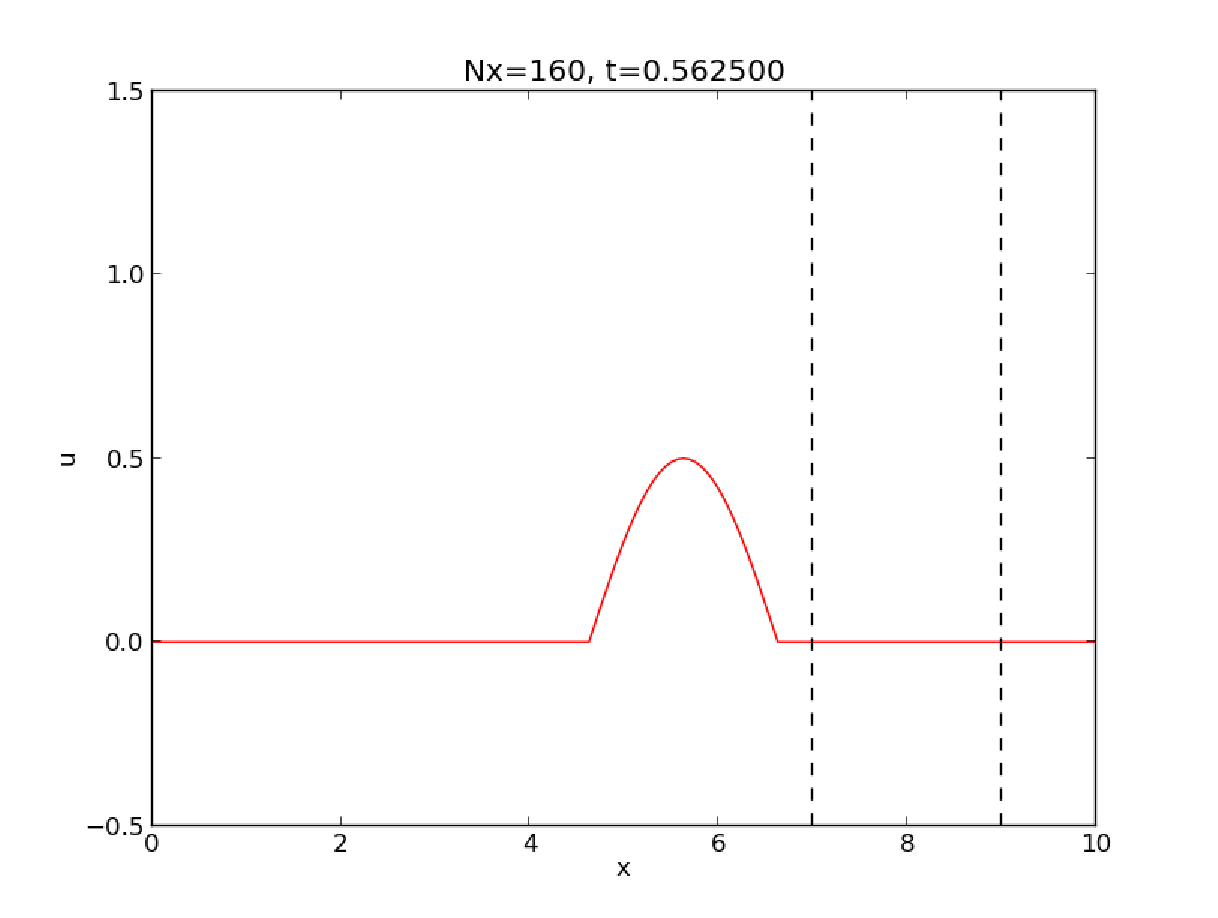
\includegraphics[width=0.7\linewidth]{../doc/src/manual/fig/wave1D.pdf}}



Figure~\ref{fig1} has a caption.


\begin{figure}[t]
  \centerline{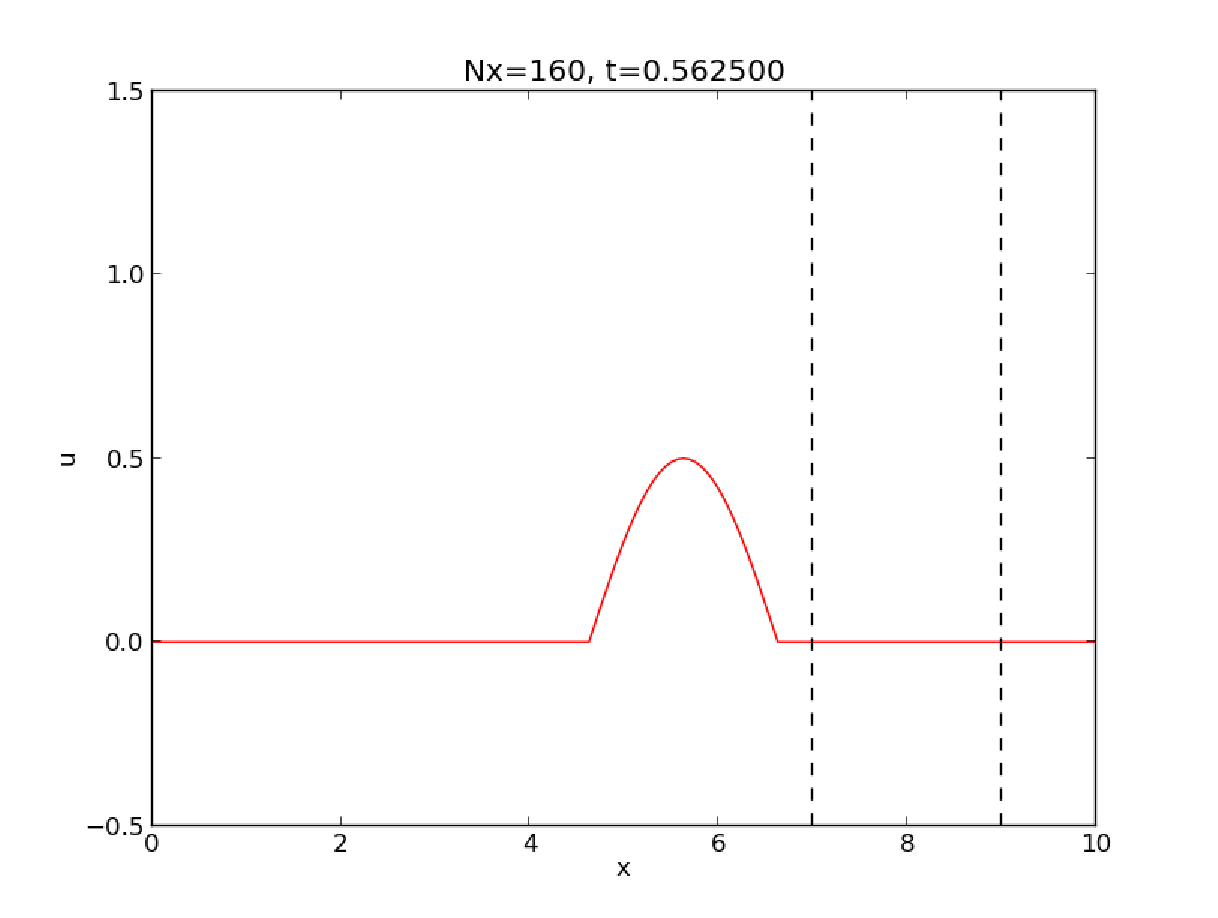
\includegraphics[width=0.7\linewidth]{../doc/src/manual/fig/wave1D.pdf}}
  \caption{
  Figure with caption. \label{fig1}
  }
\end{figure}
%\clearpage % flush figures fig1


Here is a YouTube movie:


\begin{doconce:movie}
\refstepcounter{doconce:movie:counter}
\begin{center}
\href{{http://www.youtube.com/embed/P8VcZzgdfSc}}{\nolinkurl{http://www.youtube.com/embed/P8VcZzgdfSc}}
\end{center}
\end{doconce:movie}



\begin{doconce:movie}
\refstepcounter{doconce:movie:counter}
\begin{center}
% link to external viewer
\href{run:../doc/src/manual/mov/wave.webm}{\nolinkurl{../doc/src/manual/mov/wave.webm}}
\end{center}

\begin{center}  % movie caption
Movie \arabic{doconce:movie:counter}: Movie on the hard disk: 1D wave motion.
\end{center}
\end{doconce:movie}


% !split
\section{Test of math, code, admons, quiz}

\subsection{Math}

We have

\begin{equation}
F = \int_a^b f(x)dx.
\end{equation}

\subsection{Code}

We can do the integral by

\begin{Verbatim}[numbers=none,fontsize=\fontsize{9pt}{9pt},baselinestretch=0.95,xleftmargin=2mm]
>>> from sympy import *
>>> x = 'symbols('x')
>>> f = x*sin(x)*exp(-x)
>>> integrate(f, x(0, 4))
-2*exp(-4)*sin(4) - 5*exp(-4)*cos(4)/2 + 1/2
\end{Verbatim}

Or we can do it numerically via the Trapezoidal rule:

\begin{Verbatim}[numbers=none,fontsize=\fontsize{9pt}{9pt},baselinestretch=0.95,xleftmargin=2mm]
import numpy

def trapezoidal(f, a, b, n=100):
    """Integrate f from a to b with 100 intervals."""
    x = numpy.linspace(a, b, n+1)
    F = (b-a)/float(n)*(numpy.sum(f(x)) - 0.5*(f(a) + f(b)))
    return F

def f(x):
    return x*numpy.sin(x)*numpy.exp(-x)

print trapezoidal(f, 0, 4)
\end{Verbatim}

\subsection{Admonitions}


\begin{question_mdfboxadmon}[Question.]
How do adminitions look like? That depends on the output format and
what type of admon design in the format one has chosen.
\end{question_mdfboxadmon}




\begin{warning_mdfboxadmon}[White space is important!]
Many DocOnce errors arise from wrong use of white space. The white space
is not as critical as in reStructuredText, but is not ignored either,
as in {\LaTeX} and HTML.
\end{warning_mdfboxadmon}



% ------------------- end of main content ---------------


% #ifdef PREAMBLE
\printindex

\end{document}
% #endif

